\documentclass[12pt]{article}
\usepackage{amsmath}
\usepackage{graphicx}
\usepackage{hyperref}
\usepackage{listings}
\usepackage{color}
\usepackage{float}
\usepackage[latin1]{inputenc}

\definecolor{dkgreen}{rgb}{0, 0.6, 0}
\definecolor{gray}{rgb}{0.5, 0.5, 0.5}
\definecolor{mauve}{rgb}{0.58, 0, 0.82}

\lstdefinelanguage{pctl}
  {
    morekeywords={label,R,F,min,max},
    morekeywords=[2]{phase},
    sensitive=false,
    keywordstyle=[2]\color{red},
    morecomment=[l]{//},
    morestring=[b]"
  }

\lstdefinelanguage{prism}
  {
    keywords={rewards,endrewards},
    otherkeywords={0,1,2,3,4,5,6,7,8,9},
    morekeywords=[2]{kA,kB,receiveA,receiveB,phase,party,n,b,N,L,K},
    keywordstyle=\color{blue},
    keywordstyle=[2]\color{red},
    sensitive=false,
    morecomment=[l]{//},
    morestring=[b]",
    morestring=[r]'
  }

\lstset{
  frame=t,
  language=prism,
  aboveskip=3mm,
  belowskip=3mm,
  showstringspaces=false,
  columns=flexible,
  basicstyle={\small\ttfamily},
  numbers=none,
  numberstyle=\tiny\color{gray},
  keywordstyle=\color{blue},
  commentstyle=\color{dkgreen},
  stringstyle=\color{mauve},
  breaklines=true,
  breakatwhitespace=true,
  tabsize=3
}

\title{Probabilistic Model Checking - Practical 2}
\date{}
\begin{document}
\maketitle

\section {}
\begin{lstlisting}[caption=EGL3 Changes]
// A sends bth bit of nth secret (for  n=1..N), move to B
[receiveB] phase=2 & party=1 & n<N -> (party'=2);
// B sends bth bit of nth secret (for  n=1..N-1), move to next secret and A
[receiveA] phase=2 & party=2 & n<N-1 -> (n'=n+1) & (party'=1);
// B sends bth bit of Nth secret, moves to next bit, 1st secret, and back to A
[receiveA] phase=2 & party=2 & n=N-1 & b<L -> (party'=1) & (n'=0) & (b'=b+1);
// B sends bth bit of Nth secret, move to next phase (N+1..2N), and back to A
[receiveA] phase=2 & party=2 & n=N-1 & b=L -> (party'=1) & (n'=0) & (b'=1) & (phase'=3);

// A sends bth bit of nth secret (for  n=N+1..2N-1), move to B
[receiveB] phase=3 & party=1 & n<N -> (party'=2);
// B sends bth bit of (N+n)th secret (for  n=N+1..2N-1), move to next secret and A
[receiveA] phase=3 & party=2 & n<N-1 -> (n'=n+1) & (party'=1);
// B sends bth bit of (N+n)th secret, next bit, 1st secret, and back to A
[receiveA] phase=3 & party=2 & n=N-1 & b<L -> (party'=1) & (n'=0) & (b'=b+1);
// B sends bth bit of (N+n)th secret, and protocol is now finished.
[receiveA] phase=3 & party=2 & n=N-1 & b=L -> (phase'=4);
\end{lstlisting}

\clearpage

\begin{lstlisting}[caption=EGL4 Changes]
// A sends ith bit of 1st secret to B
[receiveB] phase=2 & party=1 & n=0 -> (party'=2);

// B sends ith bit of (0..N-1)th secret to A
[receiveA] phase=2 & party=2 & n<N-1 -> (n'=n+1);
// B sends (1..L-1)th bit of last secret to A, switches back to A
[receiveA] phase=2 & party=2 & n=N-1 & N>1 -> (n'=1) & (party'=1);
// B sends last bit of the last secret to A, and switches back to A
[receiveA] phase=2 & party=2 & n=N-1 & N=1 & b<L -> (n'=0) & (b'=b+1) & (party'=1);
// B sends last bit of the 1st AND last secret to A, next phase
[receiveA] phase=2 & party=2 & n=N-1 & N=1 & b=L -> (n'=0) & (b'=1) & (party'=1) & (phase'=3);
// A sends ith bit of (1..N-1)th secret to B
[receiveB] phase=2 & party=1 & n>0 & n<N-1 -> (n'=n+1);
// A sends (1..L-1)th bit of last secret to B, moves to next bit
[receiveB] phase=2 & party=1 & N>1 & n=N-1& b<L-> (n'=0)&(b'=b+1);
// A sends the last bit of last secret to B, moves to next phase
[receiveB] phase=2 & party=1 & N>1 & n=N-1 & b=L -> (n'=0) & (b'=1) & (phase'=3);

// A sends ith bit of (N+1)th secret to B
[receiveB] phase=3 & party=1 & n=0 -> (party'=2);

// B sends ith bit of (N..2N-1)th secret to A
[receiveA] phase=3 & party=2 & n<N-1 -> (n'=n+1);
// B sends (1..L-1)th bit of last secret to A, switches back to A
[receiveA] phase=3 & party=2 & n=N-1 & N>1 -> (n'=1) & (party'=1);
// B sends last bit of the last secret to A, and switches back to A
[receiveA] phase=3 & party=2 & n=N-1 & N=1 & b<L -> (n'=0) & (b'=b+1) & (party'=1);
// B sends last bit of the 1st AND last secret to A, next phase
[receiveA] phase=3 & party=2 & n=N-1 & N=1 & b=L -> (phase'=4);
// A sends ith bit of (1..N-1)th secret to B
[receiveB] phase=3 & party=1 & n>0 & n<N-1 -> (n'=n+1);
// A sends (1..L-1)th bit of last secret to B, moves to next bit
[receiveB] phase=3 & party=1 & N>1 & n=N-1 & b<L->(n'=0)&(b'=b+1);
// A sends last bit of last secret to B, and moves to next phase
[receiveB] phase=3 & party=1 & N>1 & n=N-1 & b=L -> (phase'=4);
\end{lstlisting}

\section{}

\begin{figure}[H]
  \caption{E[messages until both parties know a pair]}
  \centering
    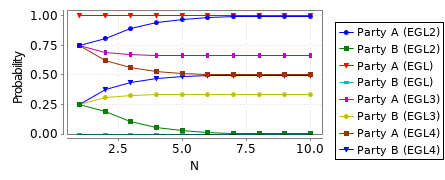
\includegraphics[width=1\textwidth]{egl1234_prob_party_disadvantaged.png}
\end{figure}

\section{}

\begin{lstlisting}[caption=Reward structure for E{[messages until both parties know a pair]}]
rewards "messages_needed"
	[receiveA] !(kB & kA) : 1;
	[receiveB] !(kB & kA) : 1;
endrewards
\end{lstlisting}

\begin{lstlisting}[caption=Property for calculating E{[messages until both parties know a pair]},language=pctl]
R{"messages_needed"}=? [ F phase=4 ]
\end{lstlisting}

\clearpage

\section{}
\begin{figure}[H]
  \caption{E[messages until both parties know a pair]}
  \centering
    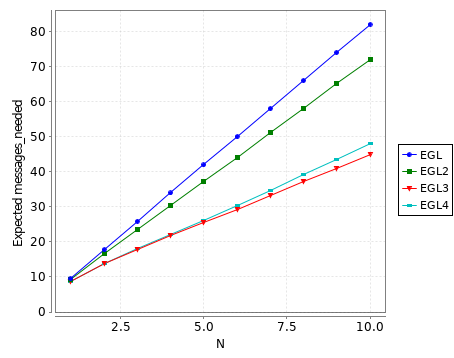
\includegraphics[width=1\textwidth]{egl1234_expected_messages_both_parties_2.png}
\end{figure}

\end{document}

